\documentclass[12pt,a4paper]{article}
\usepackage{amsfonts, amssymb, amsmath}
\usepackage{fullpage}
\usepackage{parskip} % skip a line instead of indenting
\usepackage{graphicx} % for inserting images
\usepackage{amsthm}
\usepackage{xcolor}
\usepackage{tikz} % for plot

\newtheorem*{rem}{Remark}

\title{Algorithms}
\author{R4 Cheng}
\date{\today}

\newcommand{\Remark}[1]{
  \begin{rem}
    \color{cyan}
    #1
  \end{rem}
}

\begin{document}
\maketitle

\textbf{Def.} Introduction of precise, umambiguous, and correct procedures for solving general problems

We care how many clicks in debug mode

Runtime is expressed by counting the number of steps, as funtion of \textbf{the size of the input}

Asymptotic Notations:

\begin{itemize}
  \item Big $O$: upper bound on the growth rate
  \item Little $o$: "strict" upper bound on the growth rate
  \item Big $\Omega$: lower bound on the growth rate
  \item $\Theta$: tight bound on the growth rate
\end{itemize}

$f(n)$: the runtime of an algorithm for input size $n$

$g(n)$: a simplified function without constants, lower order terms, e.g. $n^2$, $n \log n$

\textbf{Big-O Definition}: It is said $f(n) = O(g(n)) \iff$ there exists a constant $c > 0$ and $n_0 > 0$ such that
$$f(n) \leq c \cdot g(n) \text{ for all } n \geq n_0$$

\textbf{Little-o Definition}:
$$f(n) = o(g(n)) \iff \lim_{n \to \infty} \frac{f(n)}{g(n)} = 0$$

\textbf{Big-$\Omega$ Definition}: It is said $f(n) = \Omega(g(n)) \iff$ there exists a constant $c > 0$ and $n_0 > 0$ such that
$$f(n) \geq c \cdot g(n) \text{ for all } n \geq n_0$$

\subsubsection*{Caveats about constants}

For $\log_4(n)$, is 4 ignorable? No, it matters

\Remark{$log_a(x) = log_a blog_b(x)$}

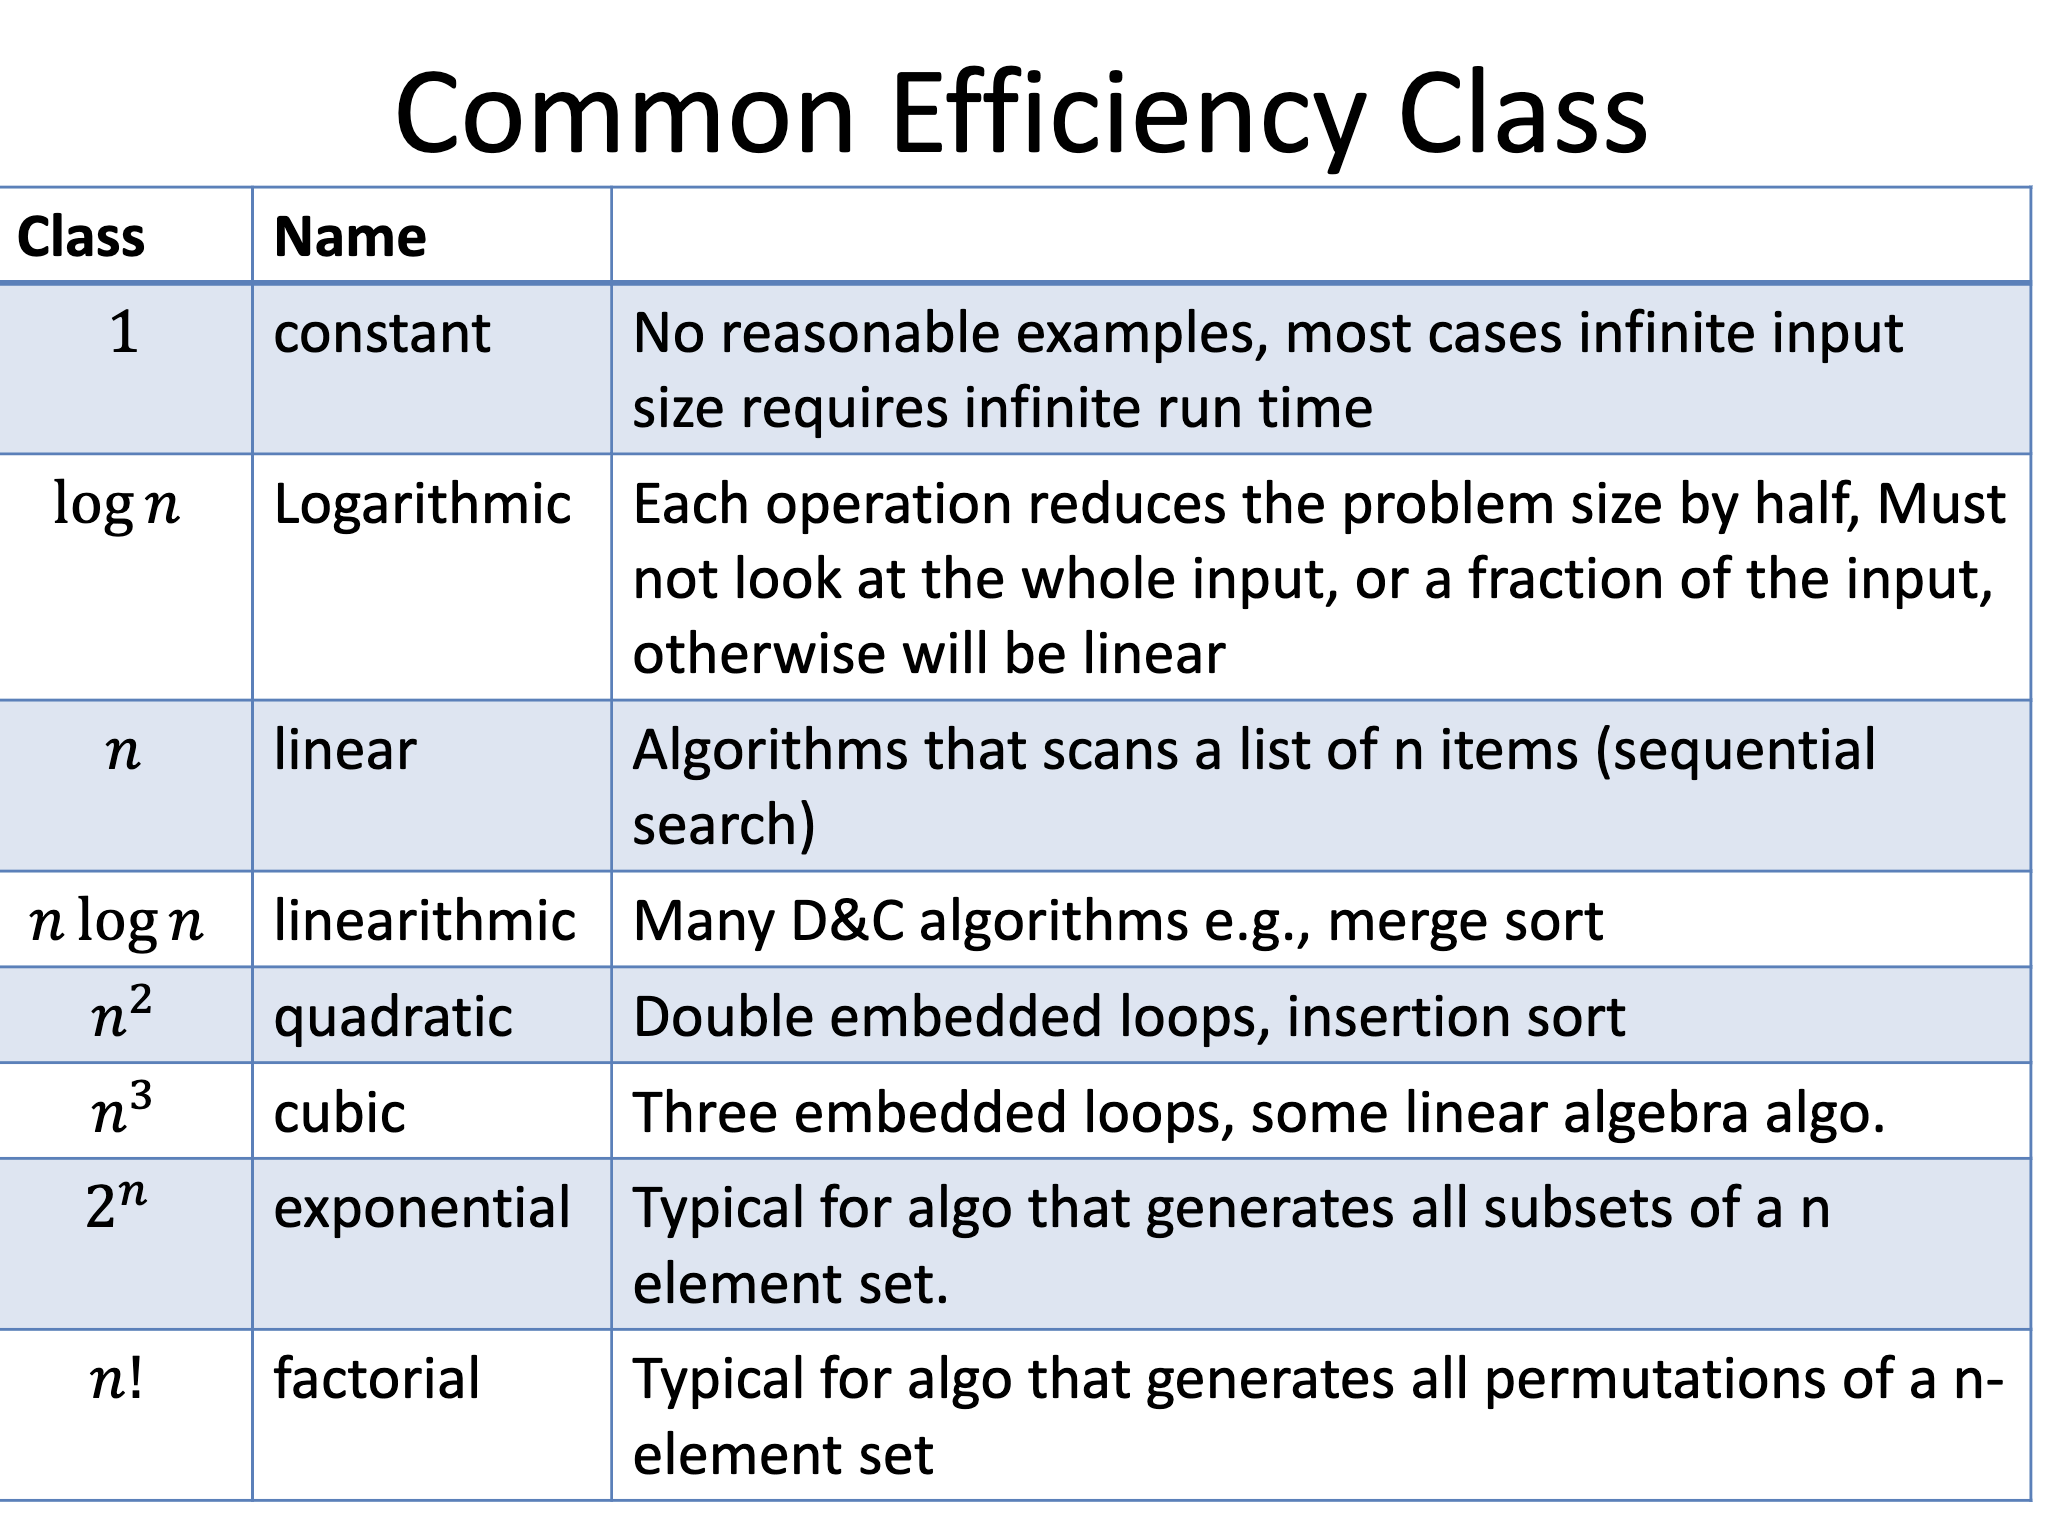
\includegraphics[width=\textwidth]{./images/common_efficiency_class.png}

\subsection*{Merge Sort}

\[T(n) = 2T(\frac{n}{2}) + 2n + c\]

\Remark{$2n$: compare and copy n elements $= 2n$}

\textbf{Proof}

\[T(n) = 2T(\frac{n}{2}) + 2n + c\]
\[\Rightarrow T(\frac{n}{2}) = 2T(\frac{n}{4}) + (n + c)\]
\[\Rightarrow T(\frac{n}{4}) = 2T(\frac{n}{8}) + (\frac{n}{2} + c)\] Bring in $T(\frac{n}{2})$
\[\Rightarrow T(n) = 2\{2T(\frac{n}{4}) + (n + c)\} + 2n + c\]
\[= 2^2T(\frac{n}{2^2}) + 2 \cdot 2n + c\] Bring in $T(\frac{n}{4})$
\[= 2^2\{2T(\frac{n}{8}) + (\frac{n}{2} + c)\} + 2 \cdot 2n + c\]
\[= 2^3T(\frac{n}{2^3}) + 3 \cdot 2n + c\]
\[\Rightarrow T(n)= 2^kT(\frac{n}{2^k}) + k \cdot 2n + c\]

Since $T(1) = 1$, $\frac{n}{2^k} = 1 \Rightarrow k = \log_2(n)$

\[\Rightarrow T(n) = n \cdot 1 + \log_2(n) \cdot 2n + c\]
\[\Rightarrow T(n) = O(nlogn) \]


\end{document}